\documentclass[a4paper]{report}

\usepackage[a4paper, total={5.75in, 10in}]{geometry}
\usepackage[english]{babel}
\usepackage[utf8]{inputenc}
\usepackage[export]{adjustbox}
\usepackage{amsmath}
\usepackage{graphicx}
\usepackage{wrapfig}
\usepackage{subcaption}
\usepackage{epigraph}
\usepackage{multirow}
% pour la modification du style des pages (numérotation)
%\usepackage{fancyhdr}



\graphicspath{ {images/} }

\title{\LARGE{RAPPORT DE PROJET}}
\author{\textsc{Dressayre} Nicolas, \textsc{Sylla} Cheick}
\date{\today}
\makeatletter

%\pagestyle{fancy}
%\fancyhf{}

%\rhead{RAPPORT DE STAGE__________}
%\lhead{Présentation}
%\renewcommand{\headrulewidth}{0pt}
%\rfoot{Page \thepage \hspace{1pt} sur n}


\begin{document}
	
	
	% --------------------------------------------------- PAGE DE GARDE
		\enlargethispage{2cm}
		
		\begin{center}
			%logos
			
\includegraphics[width=6cm]{logo_um.png}
			
			%titre
			\vspace*{3cm}
			\Huge{\@title}\\
			
			
			\large{\textbf{Faculté des sciences de Montpellier}}\\
			%\vspace*{0.5cm}
			Département Électronique, Énergie électrique et Automatique\\
			du 17 Janvier au 30 Mai 2022 \\
			
			%formation
			\vspace*{1cm}
			\large{Présenté pour obtenir la}\\
			\vspace*{0.5cm}
			\large{\textbf{Licence Générale}}\\
			\large{\textbf{Électronique, Énergie électrique et Automatique}}\\
			%\vspace*{0.5cm}
			%\large{A l'Institut Universitaire de Technologie de Tarbes}\\
			
			%auteur
			\vspace*{1cm}
			\large{Par}\\
			\vspace*{0.5cm}
			\large{\@author} 
			
			\vspace*{1cm}
			\large{Devant}\\
			
			\vspace*{1cm}
			\large{\textbf{Enseignent Référent}}\\
			\large{Aurore Vicet}\\
			Maître de conférences - HDR / Associate professor\\
			
			\vspace*{1cm}
			\large{\textbf{Membre du jury ...}}\\
			\large{m. Dupont}\\
			Lorem ipsum dolor sit amet\\
			
			%	\begin{tabular}{lr}
			%	\textbf{Maître de stage dans l'entreprise}					& \textbf{Enseignant Référent} 	\\
			%	Nathalie Yerle 											& Fabien Lacressonniere 			\\
			%	  Traction Control / Software Skill Leader 					& Maître de Conférences à l'IUT de Tarbes	\\
			%	\end{tabular}
					
		\end{center}
	\pagebreak % PAGE BREAK !!! ------------------------------------------------- PAGE BREAK !!!		
	% --------------------------------------------------- FIN DE PAGE DE GARDE
	
	% --------------------------------------------------- DÉBUT ABSTRACT
		
		\begin{center}
			\textbf{Introduction}
		\end{center}
		{\huge C}e document rapporte mon expérience et mes travaux au cours du projet de réalisé en troisième énnée de licence générale en Électronique, Énergie électrique et Automatique réalisée à la Faculté des Sciences de Montpellier.\\
		
		L'objectif premier de ce projet est de ...

		
		\vspace*{3cm}
		
		\begin{center}
			\textbf{Remerciements}
		\end{center}
	
		{\huge N}ous tenons à remercier toutes les personnes qui nous ont apporté leur aide lors ce projet et pendant la rédaction de ce rapport.\\

En premier lieu, nous voudrons exprimer mes remerciements à ...
Nous tenons aussi à remercier ...\\

Nous saisissons cette occasion pour remercier les enseignants du département EEA, notamment.... Tous ont garanti non seulement le bon déroulement du projet, mais aussi de l'année universitaire.\\

%Je remercie également l'équipe Contrôle Commande, en particulier Didier Colin et Alexandre Lamoulie qui ont su répondre à mes questions et procurer les informations nécessaires lorsque j'ai rencontré des difficultés.\\

Pour finir, un grand merci à... %/mes amis et collègues qui m'ont guidé pour la rédaction de ce rapport.
		
%		\vspace*{3cm}
%		\begin{center}
%			\textit{"Les vieux deviennent cons. \\ Les jeunes deviennent vieux".}\\
%			Alexandre L. , 2021
%		\end{center}

	% --------------------------------------------------- FIN ABSTRACT
	
	% --------------------------------------------------- DÉBUT REMERCIEMENTS 
	%remerciements sur meme page que abstract
	% --------------------------------------------------- FIN REMERCIEMENTS
	
	% --------------------------------------------------- DÉBUT SOMMAIRE
	\renewcommand*\contentsname{Sommaire} % changement du titre de la tableofcontents
	\tableofcontents
	\pagebreak
	% --------------------------------------------------- FIN SOMMAIRE
	
	% --------------------------------------------------- DÉBUT LISTE TAB/FIG
	% --------------------------------------------------- FIN LISTE TAB/FIG
	
	% --------------------------------------------------- DÉBUT GLOSSAIRE
	% --------------------------------------------------- FIN LISTE GLOSSAIRE
	
	
	% --------------------------------------------------- DÉBUT DÉVELOPPEMENT
	
	\renewcommand{\chaptername}{Partie} % changement du titre des chapitres en "parties"
	\chapter{Présentation de la spectroscopie et de la QEPAS}
	Afin de mieux appréhender le sujet, nous avons résumé le fonctionnement et les principes physiques utilisés pour la mise en œuvre de la spectroscopie et plus particulièrement de la spectrophotométrie acoustique améliorée par quartz.
	\section{Spectroscopie Classique}
	De manière générale, la spectroscopie est définie comme le champs d'études qui mesure et interprète les spectres électromagnétiques résultants de l'interaction entre une onde électromagnétique et un matériau à étudier.
	Historiquement, c'est au milieu du $XVII^{e}$ siècle que Isaac Newton montre que la lumière blanche du soleil peut être dispersée en une série continue de couleurs. Newton utilise le terme "spectre" pour décrire ce phénomène. Le premier spectroscope utilisait une ouverture pour définir un rayon de lumière collimaté par une lentille et finalement dispersé par un prisme (fig. \ref{illus:newton}). Cette analyse de la lumière était la première étape dans l'évolution de la spectroscopie.\\
	\begin{figure}[h]	
		\begin{center}			
		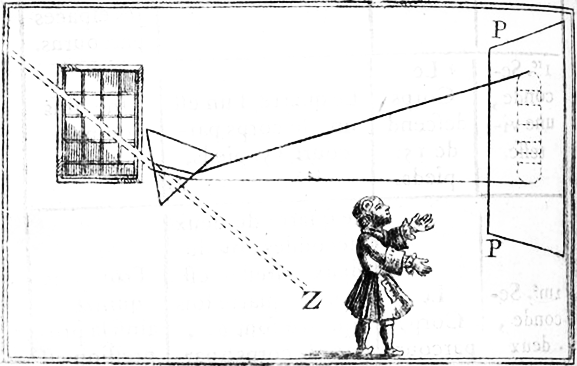
\includegraphics[width=0.6\textwidth]{spectro_newton}
		\caption{Expérience de Newton illustrée dans \textit{Élémens de la philosophie de Neuton} de Voltaire, 1738.}
		\label{illus:newton}				
		\end{center}
	\end{figure}
	Le $XIX^{e}$ siècle	a vu de nombreuses améliorations apportée à la technique. Joseph Fraunhofer a étendu la découverte de Newton en remplaçant le prisme par un réseau de diffraction comme élément de dispersion. Le réseau de diffraction, reposant sur l'interférence des rayons lumineux pour produire un paterne de diffraction, permet la mesure directe de la longueur d'onde du rayon diffracté. Cette nouvelle technique permet une résolution spectrale supérieure au prisme, Fraunhofer a ainsi pu observer de nombreuses raies sombres dans le spectre issu de la lumière du soleil.\\
	Malgré ses exploits, Fraunhofer ne comprenait pas l'origine des raies spectrales qu'il observait. C'est 33 ans après sa mort que Gustav Kirchhoff découvre que chaque élément et composé chimique a son propre spectre. Ainsi, en étudiant le spectre d'une source non connue, il est possible déterminer sa composition chimique. Kirchoff a aussi remarqué que lorsque de la lumière ayant un spectre continu passe au travers d'un gaz froid de faible densité, le résultat observé est un spectre d'absorption.\\
	Cette avancée a permis d'expliquer les raies que Fraunhofer observait sur le spectre du soleil. Elles proviennent en fait aux raies d'absorption des éléments chimiques présents dans les couches supérieures du Soleil.\\
	En se rendant compte que chaque espèce chimique a un spectre caractéristique, Kirchhoff a établit la spectroscopie comme un outil scientifique pour analyser la composition d'objets terrestres et spatiaux.
	\section{Spectroscopie d'absorption directe}
	Ce projet traite d'une variation de la spectroscopie d'absorption directe. Cette technique est utilisée pour l'analyse d'une espèce gazeuse contenue dans une cellule. La configuration classique est la suivante(fig. \ref{illus:spectro_direct}):
	
	\section{QEPAS}
		\subsection{principe de la QEPAS}
			
	\section{Mise en oeuvre a l'IES}

	\chapter{Contexte et objectifs du projet}

	
	\section{Contexte}
	Le besoin est de réaliser un appareil facilitant la mise en œuvre des manipulations QEPAS. En effet, beaucoup de matériel est nécessaire à la mise en place de cette technique et il serait bénéfique de condenser l'étage d'affichage des mesures dans un seul appareil.
	Notre projet intervient donc à la suite de la détection synchrone.
	
	\section{Objectif: Afficheur de mesure de signal QEPAS}
	L'objectif de notre projet est de représenter en temps réel l'évolution du signal d'acquisition sur graphe.
	
	\chapter{Afficheur de mesures de concentration de gaz}
	
	
	\section{Besoin technique}
	
	\section{Gestion de projet et organisation du travail}
	Le travail est réparti entre Nicolas Dressayre et Cheick Sylla. 
	
	\section{Conception}
	\subsection{architecture retenue}
	Nous avons choisi d'utiliser le SBC (single-board computer) très populaire Raspberry Pi 3B+ comme élément central de notre projet. Cet ordinateur disposant d'une sortie HDMI est entièrement capable d'effectuer un affichage graphique des mesures QEPAS. Une autre option que nous avions envisagé aurait été d'utiliser une carte à micro contrôleur: l'Arduino Uno. Cette seconde option nous aurait permis d'effectuer l'acquisition des signaux analogiques mais pas de les afficher directement. Le micro-contrôleur ATmega328 de la carte Arduino n'a pas la capacité de générer des signaux vidéo. Une façon de contourner ce problème aurait été de connecter l'Arduino à un autre ordinateur au moyen d'une liaison série, mais le volume du système complet aurait été augmenté.\\
	
	Comme les ordinateurs Raspberry Pi ne disposent pas de convertisseur analogique-numérique intégré, nous devons en ajouter un à notre système.\\
	
	L'architecture complète de notre projet est représentée dans la figure \ref{schema:archi}. Maintenant que nous connaissons tous les éléments de notre projet, nous pouvons les détailler individuellement et brièvement expliquer leur fonctionnement.
	
	\begin{figure}[h]	
		\begin{center}			
		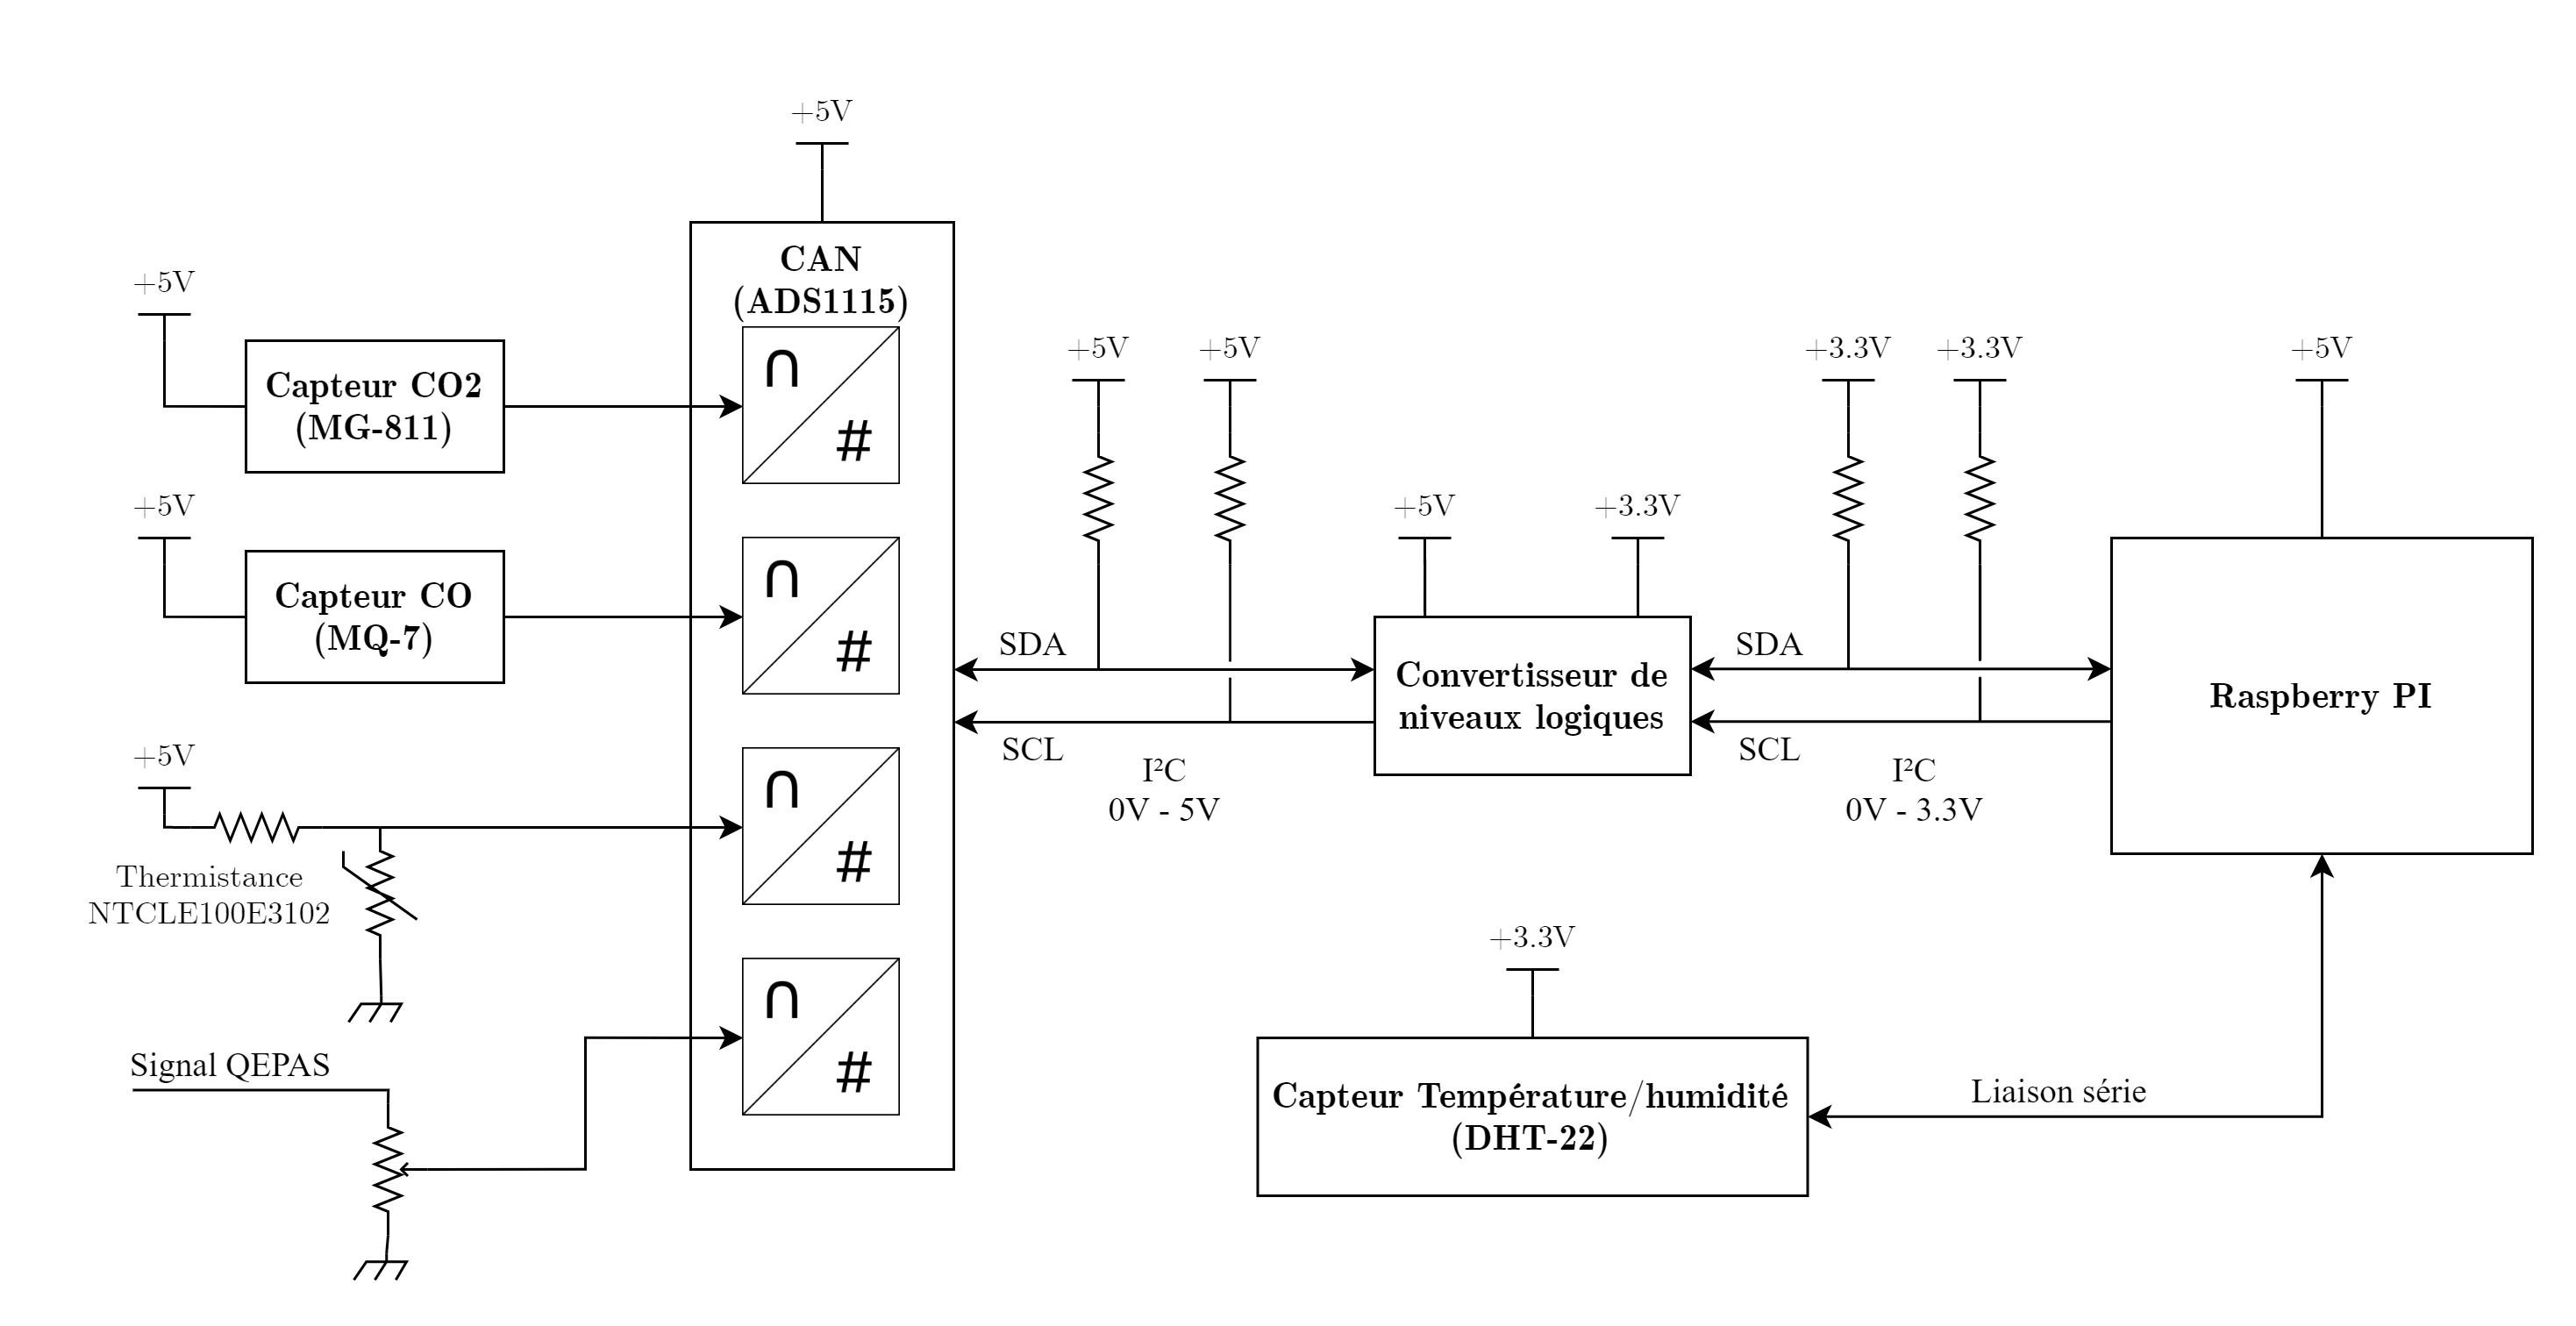
\includegraphics[width=1.2\textwidth]{systeme_global}
		\caption{Schéma de principe du projet.}
		\label{schema:archi}				
		\end{center}
	\end{figure}	

	
	\subsection{choix des composants}
	
\subsubsection{Convertisseur analogique numérique}
	Nous avons fait le choix d'utiliser un module (nom commercial KY-053) intégrant un convertisseur ADS1115. Ce composant développé par Texas Instruments a été rendu populaire par l'entreprise Adafruit qui a conçu le module ainsi que des librairies pour les plateformes Arduino et Raspberry Pi.\\
	Les principales caractéristiques du module sont résumés dans le tableau \ref{tab:ads1115}

\begin{table}[]
\centering
\begin{tabular}{|l|ll|l|}
\hline
 & \multicolumn{1}{l|}{minimum} & maximum & \multirow{7}{*}{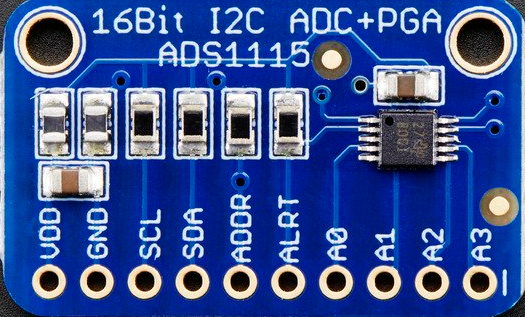
\includegraphics[width=0.3\textwidth]{ads1115}} \\ \cline{1-3}
Tension d'alimentation          & \multicolumn{1}{l|}{2V}         & 5.5V       &  \\ \cline{1-3}
Taux d'échantillonnage          & \multicolumn{1}{l|}{8 Hz}       & 860 Hz     &  \\ \cline{1-3}
Résolution                      & \multicolumn{2}{c|}{16 Bits (65536 valeurs)} &  \\ \cline{1-3}
Nombre d'entrées analogiques    & \multicolumn{2}{c|}{4}                       &  \\ \cline{1-3}
Tension des entrées analogiques & \multicolumn{1}{l|}{0.256 V}    & 6.144 V    &  \\ \cline{1-3}
Mode de communication numérique & \multicolumn{2}{c|}{I²C}                     &  \\ \hline
\end{tabular}
\caption{Principales caractéristiques de l'ADS1115}
\label{tab:ads1115}
\end{table}

\subsubsection{Capteur de dioxyde de carbone SEN-0159}
	Peu de capteurs de CO2 sont disponibles sur le marché. Nous avons fait le choix d'utiliser le SEN0159, un module produit par DFRobot intégrant un capteur électrochimique MG-811 Winsen, un fabricant chinois de capteurs dont les produits sont souvent utilisés dans les projets de domotique. En plus du capteur, le module comprend un amplificateur de signal de sortie, un circuit de chauffe pour garantir une température constante de l'élément de détection.\\
	
\begin{table}[]
\centering
\begin{tabular}{|l|cl|l|}
\hline
\multicolumn{1}{|c|}{} & \multicolumn{1}{c|}{minimum} & \multicolumn{1}{c|}{maximum} & \multirow{7}{*}{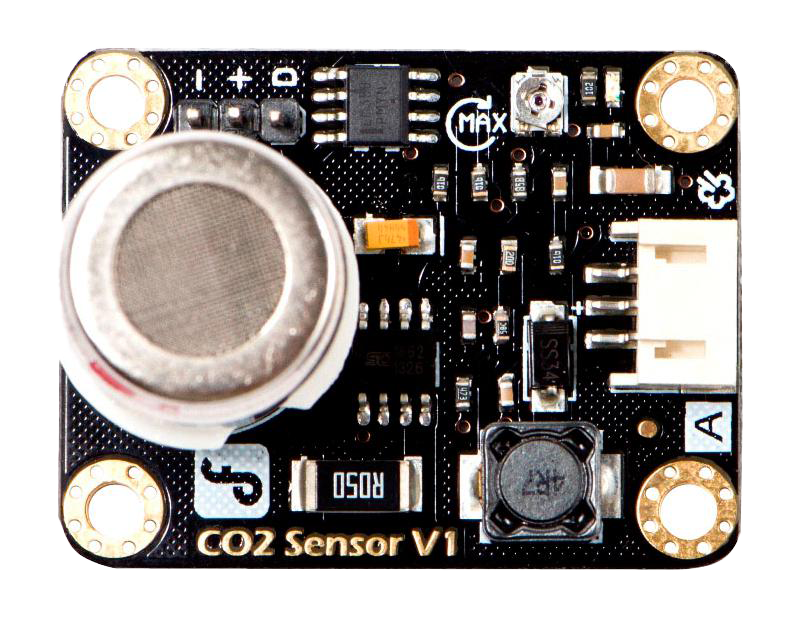
\includegraphics[width=0.25\textwidth]{sen0159}} \\ \cline{1-3}
Espèce détectée        & \multicolumn{2}{c|}{Dioxyde de carbone} &  \\ \cline{1-3}
Tension d'alimentation & \multicolumn{1}{c|}{3.5V}   & 5.0V      &  \\ \cline{1-3}
Tension de sortie      & \multicolumn{1}{c|}{2.7V}   & 4.7V      &  \\ \cline{1-3}
Type de capteur        & \multicolumn{2}{c|}{électrochimique}    &  \\ \cline{1-3}
Plage de mesure        & \multicolumn{1}{c|}{0 ppm}  & 10000 ppm &  \\ \cline{1-3}
Précision              & \multicolumn{2}{c|}{±100ppm à 400ppm}   &  \\ \hline
\end{tabular}
\caption{Principales caractéristiques du SEN-0159}
\label{tab:SEN0159}
\end{table}

\subsubsection{Capteur de monoxyde de carbone: SEN-MQ7}
	Nous avons aussi utilisé un capteur de la marque Winsen pour notre capteur de monoxyde de carbone. Il s'agit du capteur MQ7 monté sur le module SEN-MQ7 fabriqué par Joy-IT
\subsubsection{Capteur de température / humidité: DHT 22}
	Contrairement aux deux capteurs de gaz, le capteur de température DHT 22 n'a pas besoin de convertisseur analogique numérique puisque ce dernier intègre son propre micro-contrôleur et communique via un protocole série unifilaire. En plus de la température, le DHT 22 permet aussi une mesure de l'humidité ambiante et revoie une valeur en pour cents. D'un point de vue logiciel, ce capteur est très bien supporté et une librairie développée par Adafruit est disponible. Contrairement au convertisseur analogique numérique, le DHT 22 n'est capable de fournir une mesure que toutes les deux secondes.
	
\subsubsection{Convertisseur niveaux logiques}


	\subsection{éléments logiciels}
Maintenant que la partie matérielle du projet est établie et que chaque composant a été décrit, nous réalisons le programme Python permettant de lire les capteurs, de convertir les tensions lues et d'afficher les résultats sur l'écran de la Raspberry Pi.\\
Cette partie du projet a été gérée en totalité sous la forme d'un dépôt GitHub disponible à l'adresse suivante:
\begin{center}
	\texttt{https://github.com/118DRESNI/projet\_l3}
\end{center}

La première étape de programmation a été de tester individuellement les capteurs à notre disposition. Le plus simple à mettre en oeuvre est le DHT22.
	\subsection{modélisation du boitier}
	
	\section{Réalisation}
	\subsection{prototypage sur breadboard}

	\begin{figure}[h]	
		\begin{center}			
		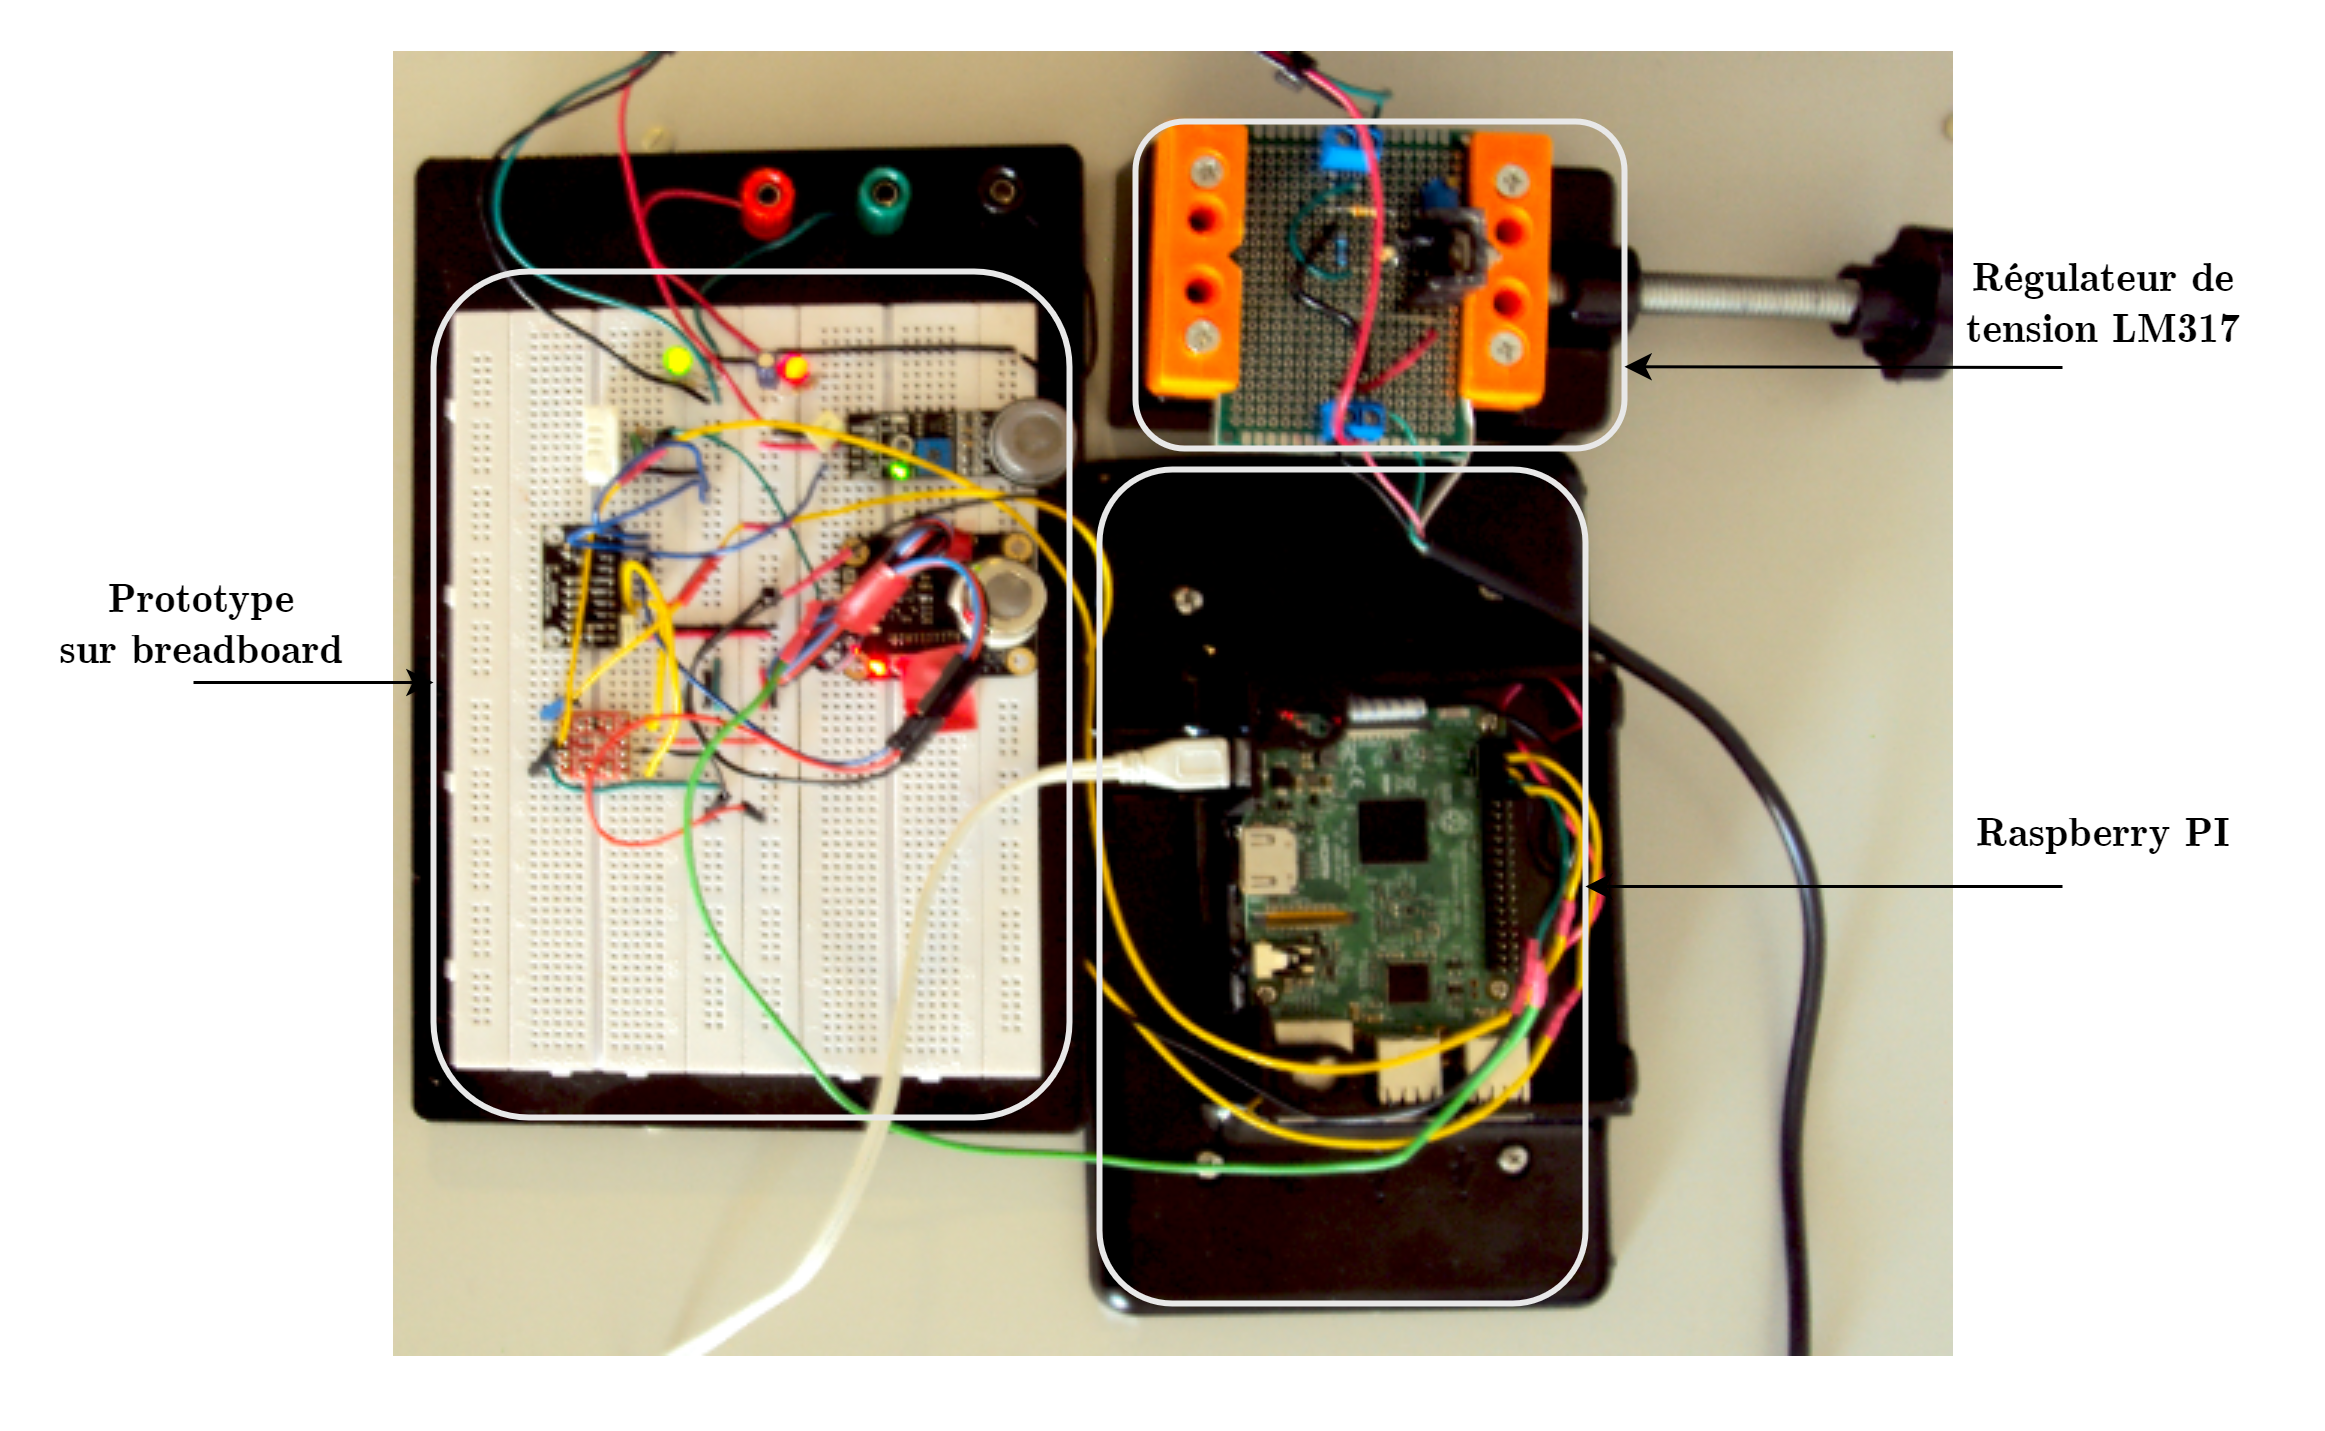
\includegraphics[width=1.1\textwidth]{schema_manip}
		\caption{Prototype complet.}
		\label{schema:manip}				
		\end{center}
	\end{figure}

	\subsection{tests préliminaires}
	\subsection{impression du boitier et assemblage}
	
	\section{conclusion, difficultés rencontrées}

	\chapter{Comparaison des performances entre QEPAS et capteurs du commerce}
	\section{Étalonnage des capteurs MQx}
	\subsection{méthode employée}
	\subsection{déroulement}
	\subsection{conclusion (comparaison avec datasheet ?)}
	
	\section{Mesures avec les deux techniques}
	\subsection{méthode employée}
	\subsection{déroulement}
	\subsection{conclusion}
	

	% --------------------------------------------------- FIN DÉVELOPPEMENT	
	\chapter{Valorisation du projet par rapport a la poursuite d'études}
	% --------------------------------------------------- DÉBUT CONCLUSION
	
		Ce projet nous a permit de réaliser... \\
		Nous avons pu mettre en œuvre des connaissances acquises en L3 EEA.\\
	
	%%	Pour finir, nous tenons à dire que nous conservons une très bonne impression de cette courte expérience dans le domaine du ferroviaire.\\
 
	
	% --------------------------------------------------- FIN CONCLUSION
	\renewcommand{\bibname}{Références} % changement du titre des chapitres en "parties"
	\begin{thebibliography}{9}
		
		
		\bibitem{transfer_thermique_pspice} 
		Shuhui Li, Rajab Challoo et Robert A. McLauchlan. 
		\textit{Heat Transfer Simulation Using PSpice}.\\ 
		Conference: ASME 2003 Heat Transfer Summer Conference.\\
		DOI:10.1115/HT2003-47021
		
		\bibitem{spectro_mit} 
		\textit{The Era of Classical Spectroscopy}.\\ 
		Site web du Massachusetts Institute of Technology [En ligne] [consulté le 10 mai 2022].\\
		Disponible sur: \\\texttt{http://web.mit.edu/spectroscopy/history/history-classical.html}		
		
		\bibitem{spectro_voltaire} 
		Marie François Arouet de Voltaire. 
		\textit{Élémens de la philosophie de Neuton, donnés par Mr de Voltaire. Nouvelle édition}.\\ 
		Bibliothèque Nationale de France [En ligne]. 1738 [consulté le 10 mai 2022].\\
		Disponible sur: \\\texttt{https://gallica.bnf.fr/ark:/12148/btv1b8622062t}
		
		\bibitem{histoire_alstom} 
		\textit{Génèse et Histoire du site Alstom à Séméac}.\\
		Maire de Soues. [En ligne]. 2014 [consulté le 20 mai 2021].\\
		Disponible sur: \\\texttt{https://www.soues.com/Fichiers/pages/155333145124genese-et-histoire-du-site-alstom-a-semeac.pdf}
		
		\bibitem{ACTGV_pmcf} 
		\textit{PMCF Onduleurs}.\\
		Association des Conducteurs de Trains à Grande Vitesse. [En ligne] M.Durochat et G.Desplanques [consulté le 05 juin 2021].\\
		Disponible sur: \\\texttt{http://actgv.fr/wp-content/uploads/2012/05/PMCF-onduleur.pdf}
		
		\bibitem{ACTGV_puissance} 
		\textit{Circuits de Puissance Traction}.\\
		Association des Conducteurs de Trains à Grande Vitesse. [En ligne] M Durochat, Jean Willemin et G. Desplanques, 2016 [consulté le 03 juin 2021].\\
		Disponible sur: \\\texttt{http://actgv.fr/wp-content/uploads/2016/10/Circuit-de-Puissance-21-04-2016-dernier-travail.pdf}
		
		\bibitem{alstom_site} 
		\textit{Site officiel d'Alstom}.\\
		Site officiel d'Alstom. [En ligne] [consulté le 08 juin 2021].\\
		Disponible sur: \\\texttt{https://www.alstom.com}
		
	\end{thebibliography}
	
	
\end{document}